\documentclass[11pt,xcolor=svgnames]{beamer}
\usepackage{dsfont,natbib,setspace,changepage,multirow,times}
\mode<presentation>

% fonts
\usepackage{pbsi}

% replaces beamer foot with simple page number
\setbeamertemplate{navigation symbols}{}
\setbeamercolor{frametitle}{fg=black}
\newcommand{\theme}{\color{Maroon}}

\setbeamertemplate{footline}{
   \raisebox{5pt}{\makebox[\paperwidth]{\hfill\makebox[20pt]{\color{gray}\scriptsize\insertframenumber}}}}

\usepackage{tikz}
  
\graphicspath{{/green/Dropbox/inputs/},
{/Users/mtaddy/Dropbox/inputs/},
{/home/taddy/project/bigdata/graphs/},
{/Users/mtaddy/project/bigdata/graphs/}}

\setbeamercolor{whitebox}{bg=gray!10}

% colors
\newcommand{\bk}{\color{black}}
\newcommand{\rd}{\color{red}}
\newcommand{\fg}{\color{ForestGreen}}
\newcommand{\bl}{\color{blue}}
\newcommand{\gr}{\color{black!60}}
\newcommand{\sg}{\color{DarkSlateGray}}
\newcommand{\br}{\color{SaddleBrown}}
\newcommand{\nv}{\color{Navy}}


% common math markups
\newcommand{\bs}[1]{\boldsymbol{#1}}
\newcommand{\mc}[1]{\mathcal{#1}}
\newcommand{\mr}[1]{\mathrm{#1}}
\newcommand{\bm}[1]{\mathbf{#1}}
\newcommand{\ds}[1]{\mathds{#1}}
\newcommand{\indep}{\perp\!\!\!\perp}

% spacing and style shorthand
\setstretch{1.1}

% shorthand
\newcommand{\sk}{\vspace{.5cm}}
\newcommand{\R}[1]{{\tt \nv #1}}
\newcommand{\til}{{\footnotesize$\bs{\stackrel{\sim}{}}$}}
\DeclareSymbolFont{extraup}{U}{zavm}{m}{n}
\DeclareMathSymbol{\vardiamond}{\mathalpha}{extraup}{87}

\begin{document} 

\setcounter{page}{0}
{ \usebackgroundtemplate{
\includegraphics[height=\paperheight]{phoenix}}
\begin{frame}[plain]
\begin{center}


{\bf \Large  Big Data: Text}

\vskip 1.5cm 
Matt Taddy, University of Chicago Booth School of Business

\vskip .2cm 
\texttt{faculty.chicagobooth.edu/matt.taddy/teaching} 


\end{center}
\end{frame} }


\begin{frame}
{\theme Text}



{\bf \nv The Bag of Words Representation}

\sk Using what we  know: term frequencies as model inputs.

\vskip .25cm
Tokenization: ngrams, stopwords, info retrieval.

\vskip .25cm

Text-specific multinomial models.

\end{frame}


\begin{frame}

{\bf We'll start with a story: \theme Slant in Partisan Speech}

\sk
Gentzkow and Shapiro: What drives media slant?  Evidence from
U.S. daily newspapers ({\it Econometrica}, 2010).

\sk
Build an economic model for newspaper demand that incorporates political partisanship
(\rd Republican \bk vs
\bl Democrat\bk).
 
\begin{itemize}
\item What would be independent profit-maximizing ``slant''?
\item Compare this to slant estimated from newspaper text.
\end{itemize}

\end{frame}


\begin{frame}

\sk
\begin{center}
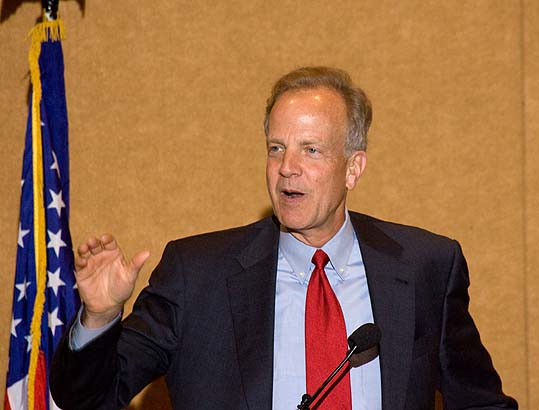
\includegraphics[width=1.7in]{../graphs/moran}
~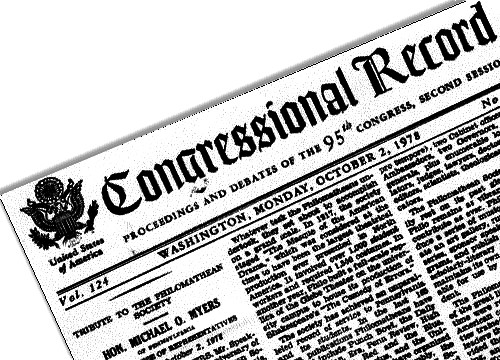
\includegraphics[width=1.75in]{../graphs/record}
\end{center}

Jerry Moran, R-KS, says ``death tax'' relatively often and his district
(Kansas 1st) voted 73\% for George W. Bush in 2004.

\begin{center}
$\bm{X_\text{text}} = f( \text{ideology}) \approx g(Y_{Bush})$

\vskip .25cm
$\bm{\Rightarrow}$ ``death tax'' is republican

\vskip .25cm
$\Rightarrow $ \theme the Wall Street Journal is slanted right.
\end{center}

\end{frame}

\begin{frame}
{What is slant?}

\sk
{\nv Text:}  phrase-counts by speaker in 109$^{th}$ US Congress
(05-06)\\
{\nv Sentiment:} two-party constituent vote-share for Bush in 2004.

\sk
Use covariance between  phrase frequencies ($f_{ij}$) and `Bush'
sentiment ($y_i$)  to build an index of partisanship
for text. 
\begin{center}\large\nv
$z^{slant}_i= \sum_j \mr{cov}(f_j, y) f_{ij}$
\end{center}

 For example, if phrase $j$ forms  a high proportion of what you
say, and usage of phrase
$j$ is correlated with Bush vote-share, then this contributes a
positive amount to your slant score.

\vskip .2cm
This is a type of {\it marginal regression}.

\end{frame}


\begin{frame}


{\bf  \Large\bsifamily Wordle} 


\sk
\begin{adjustwidth}{-.1in}{}
\vskip -.5cm
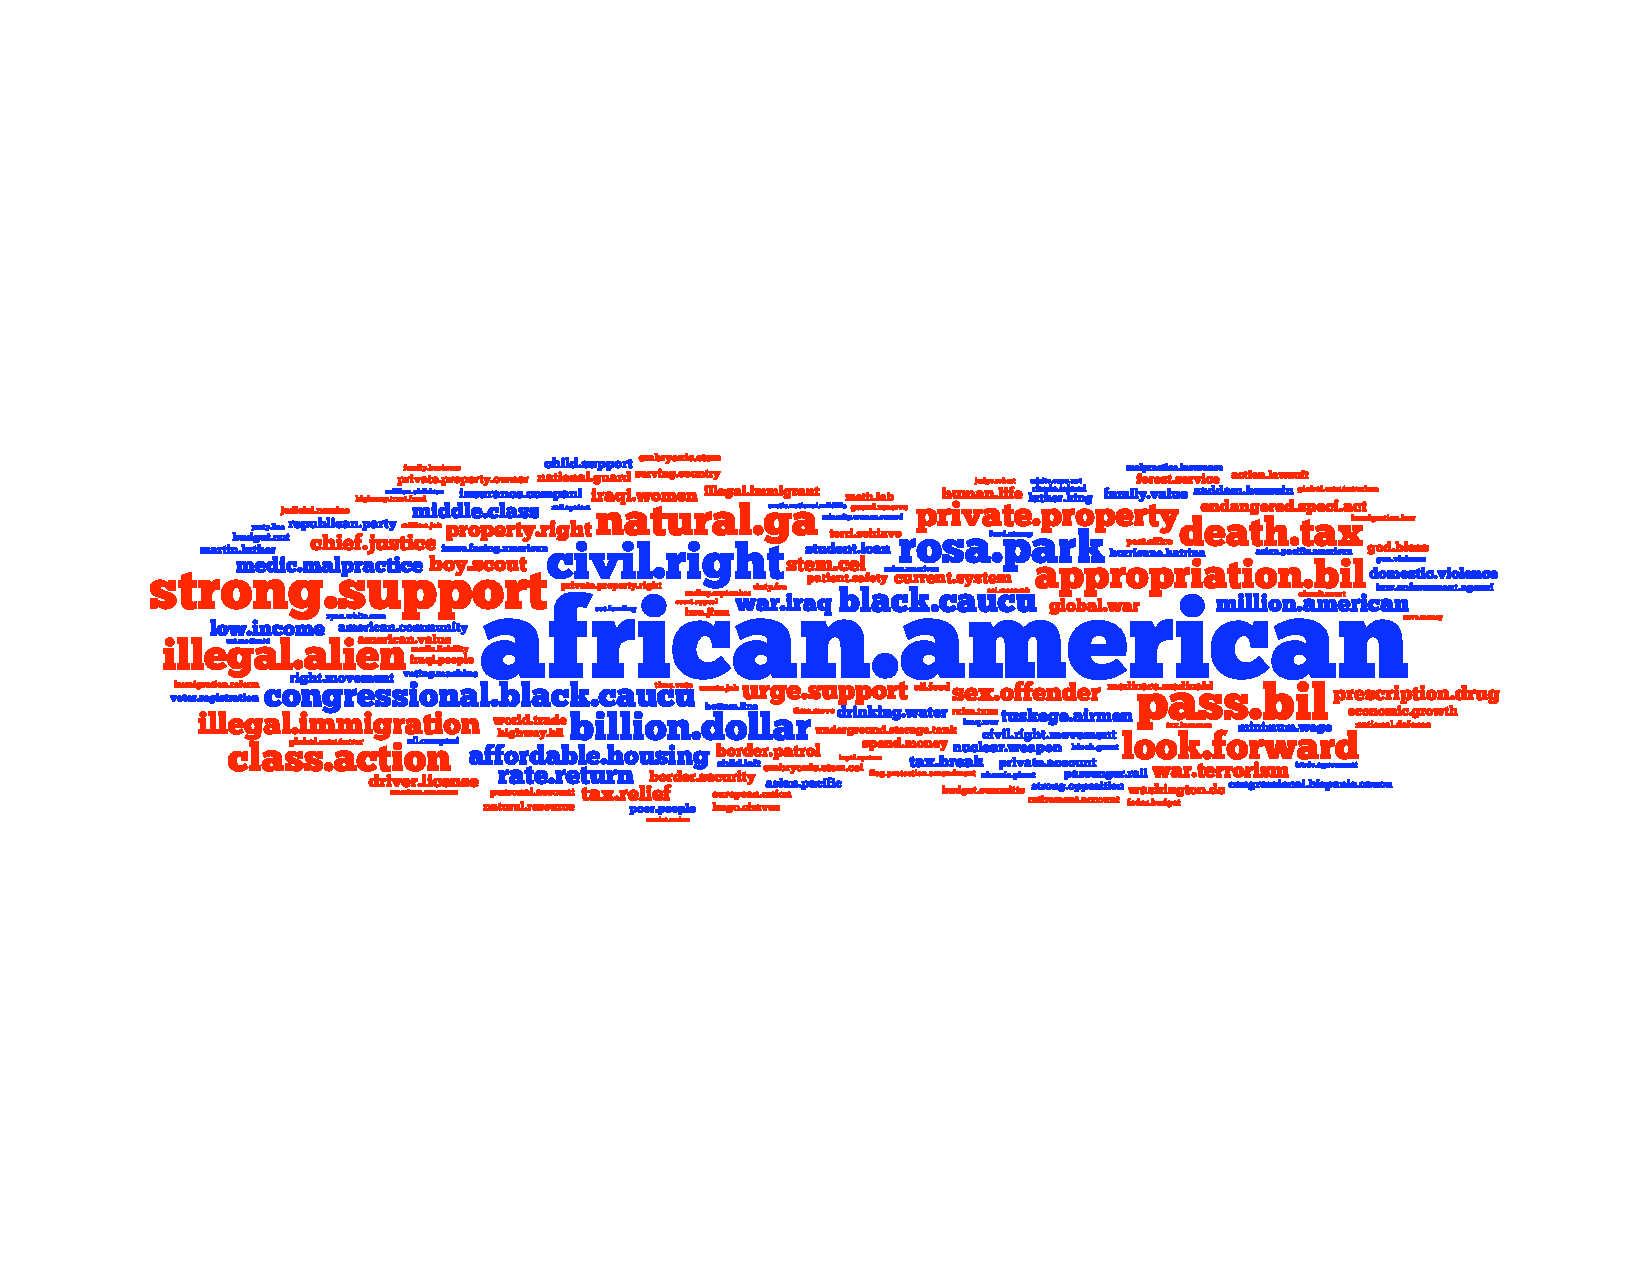
\includegraphics[width=4.5in]{../graphs/slantWrdl}
\end{adjustwidth}

\vskip .2cm
Colored by sign (\rd positive\bk, \bl negative\bk) \\ Size proportional to loading $\mr{cov}(f_j, y)$.\\

\vskip .2cm
Since $y$ is Republican vote-share, \\
big positive is a right term and big
negative is a left term.


\end{frame}


\begin{frame}

\begin{center}
{\bf Slant measure for speakers in the 109th Congress}
\vskip -.5cm
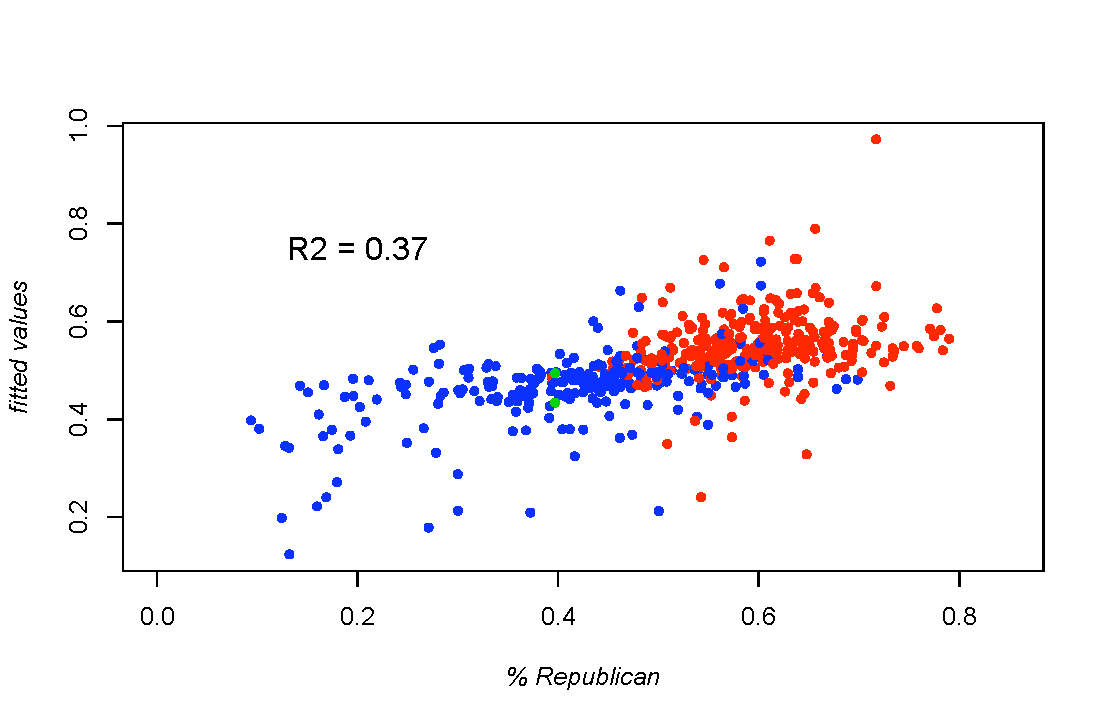
\includegraphics[width=4in]{../graphs/slant}\\
\end{center}

\vskip -.5cm
Democrats get low $z_\text{slant}$ and Republicans get high
$z_\text{slant}$.\\
\gr Do this for newspaper text and you'll get a similar picture

\end{frame}




\begin{frame}
{The Big Picture}


Text is a vast source of data for business 

\vskip .25cm
It comes connected to interesting ``author'' variables 
\begin{itemize}
\item What you buy, what you watch, your reviews
\item Group membership, who you represent, who you email
\item Market behavior, macro trends, the weather
\end{itemize}

\sk 
Opinion, subjectivity, etc.
Sentiment is {\it very} loosely defined: 

\vskip .2cm\nv
Observables linked to the variables motivating language choice

\end{frame}

\begin{frame}

{\bf \theme Text is also super high dimensional }

\vskip .25cm
 And it gets higher dimensional as you observe more speech.


\vskip .25cm
Analysis of 
phrase counts is the state of the art (hard to beat).

\sk
For example, occurances by party for some partisan terms

\vskip .25cm
{\footnotesize
\begin{tabular}{|c|c|c|c|c|c|c}
Congress & State & Party & America & Death Tax & Estate Tax & $\cdots$
\\ \hline
\multirow{2}{*}{63} & \multirow{2}{*}{\sf NM} & {\sf dem}  & 108 &
  30 & 140 & \\ &
& {\sf gop}  & 100 &
  220 & 12  &
\end{tabular}}


\sk

{\nv Basic units of data}

\begin{itemize}\bk
\item  doc-term count matrix $\bm{X}$ with rows $\bm{x}_i$.
\item  doc totals {\tt $\bm{m} = $ rowSums($\bm{X}$)} $=[m_1 \cdots m_n]$.
\item frequency matrix $\bm{F}=\bm{X}/\bm{m}$ with rows $\bm{f}_i$.
\end{itemize}

\end{frame}

\begin{frame}

{\bf We already know how to do text mining}

\vskip .1cm
Doc-term matrices can be treated like any other covariates.

\sk
{\gr Example: \bk Author Classification}

\vskip .25cm
You want to identify `authorship' from from text.

Use logistic lasso to estimate authors from
$\bm{X}$.

{\nv We've already seen this: the spam data!}
\[
\mr{logit}\left[\mr{p}({\tt spam})\right] = \alpha + \bm{f}'\bs{\beta}
\]


\theme 
It is best to regress on frequencies $\bm{F}$
rather than raw counts. 

\bk
If you think $m_i$ matters, include it as a separate variable.
\end{frame}


\begin{frame}[fragile]


{\theme We also did some text mining with the we8there reviews.}

\vskip .25cm
Topic models
\begin{semiverbatim}\nv\scriptsize\vspace{-.25cm}
summary(tpcs)\bk
Top 5 phrases by topic-over-null term lift (and usage \%):
[1] food great, great food, veri good, food veri, veri nice (13.7) 
[2] over minut, ask manag, flag down, speak manag, arriv after (11.6) 
\end{semiverbatim}

And regression
\begin{semiverbatim}\nv\footnotesize
stars <- we8thereRatings[,"Overall"]
tpcreg <- gamlr(tpcs\$omega, stars)
\gr# Effect stars from 10\% increase in topic use\bk
drop(coef(tpcreg))*0.1 
     intercept      1      2      3      4   
         0.414  0.075 -0.386  0.068  0.042   
             5      6     7     8      9     10 
         0.000  0.076 0.121 0.000 -0.134 -0.049 
\end{semiverbatim}

\end{frame}

\begin{frame}[fragile]

{\gr \it Wait: how did you get two word phrases?}

\sk

{\bf Information Retrieval and Tokenization}

\sk
A passage in `{\it As You Like It}':

\vskip .2cm
{\setstretch{1} \it
~~~ {\sg All the world's a stage,\\
~~~ and all the men and women merely players:\\
~~~ they have their exits and their entrances;\\
~~~ and one man in his time plays many parts...}
}

\vskip .2cm
What the statistician sees:

\vspace{-.4cm}{\sg
\begin{verbatim}
   world stage men women play exit entrance time 
       1     1   2     1    2    1        1    1 
\end{verbatim}}

This is the {\nv Bag-of-Words} representation of text.

\end{frame}

\begin{frame}

{\bf\theme The $n$-gram language model}

\sk 
An $n$-gram language model is one that describes a dialect through
transition probabilities on $n$ consecutive words.


\sk
An {\theme $n$-gram tokenization} counts
length-$n$ sequences of words.\\
{\sg A unigram is a word, bigrams are transitions between words.}\\
{\gr e.g., {\tt world.stage}, {\tt stage.men}, {\tt men.women}, {\tt women.play}, ...}


\sk
This can give you rich language data, but be careful:\\
$n$-gram token vocabularies are very high dimensional ($p^n$)

\sk More generally, you may have domain specific `clauses' that you wish to tokenize.
There is always a trade-off between complexity and generality.  {\theme Often best to just count words.}
\end{frame}



\begin{frame}

{\bf \theme Possible tokenization steps} 

\vskip .35cm
Remove words that are super rare {\gr (in say $<\frac{1}{2}$\%, or $<15\%$ of docs; this is application specific)}.
 For example, if {\nv Aegrotat} occurs only once, it's useless for comparing documents.

\vskip .35cm
Stemming:  `{\nv tax}' $\leftarrow$   taxing,  taxes,
  taxation, taxable, ... 

{\gr
A stemmer cuts words to their root with a mix of rules and estimation.
`Porter' is standard for English.  I don't usually stem since you can lose
meaning, but it is nice for limited data.}



\vskip .35cm
Remove a list of {\nv stop words}
containing  irrelevant tokens.

{\gr ~~~~~If, and, but, who, what, the, they, their, a, or, ...}

{\nv Be careful: one person's stopword is another's key term.}

\vskip .35cm
Convert to lowercase, drop numbers, punctuation, etc ...\\
Always application specific: e.g., don't drop {\tt :-)} from tweets.

\vskip -.25cm

\end{frame}


\begin{frame}

{\bf \theme Tokenization in R and elsewhere}

\sk 
The {\tt tm} package for R provides a set of tools\\
for cleaning and tokenizing text documents.

{\gr See class code for examples of reading
from text and pdf files.}


\sk This works well for small-to-medium sized examples, but \\to really scale up
you'll need to work out-of-memory.  \\There is an extension of {\tt tm} for Hadoop and Mapreduce.

\sk
Python is a more natural scripting language for tokenization.  There is a massive ecosystem of
tools available for dealing with foreign encodings, spell-checking, web scraping, etc...
\end{frame}

\begin{frame}

{\bf \theme Document-Term Co-occurrence Matrices}

\sk
However you tokenize, \\~~the final result is a document-term count  matrix {\nv $\bm{X}$}.

\vskip .2cm
{\gr Each row is a document, each column a token (e.g., word).}

These are the basic units of data for text analysis ($\bm{F} = \bm{X}/\bm{m}$).

\sk
Some lingo
\begin{itemize}
\item The vocabulary is {\tt colnames(X)}.
\item Vocabulary size is {\tt ncol(X)}.
\item The corpus is `all of your documents'.
\item Corpus size is {\tt nrow(X)}.
\item A token's sparsity is {\tt mean(X[,`term']==0)}.
\end{itemize}

\end{frame}



\begin{frame}

{\bf \theme Term frequencies are data like any other}

\sk In addition to lasso regression, we can do
\begin{itemize}
\item Principle components analysis
\item Partial least squares (marginal regression)
\item K-means clustering
\end{itemize}

\sk
And there are fast approximate algorithms \\{\gr (see {\tt R}'s {\tt irlba} package)}.

\vskip .2cm
Even better is to use some text-specific methods...

\end{frame}


\begin{frame}[fragile]

{\bf Example: topics on lectures from 2013 Booth 41201}

\vskip .1cm
{\gr We used {\tt tm} to read lectures from pdf and tokenize. }


\vskip .25cm
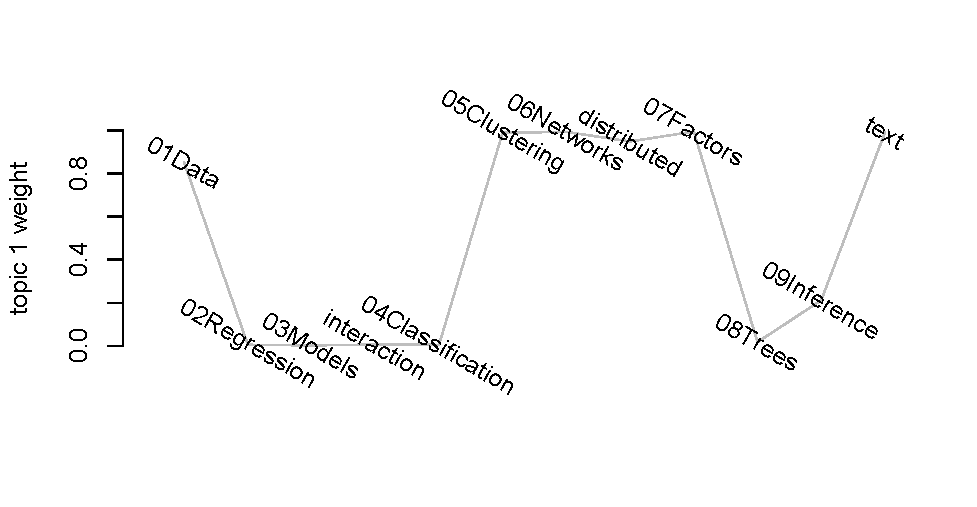
\includegraphics[width=4.25in]{../graphs/lecturesintime}

\vskip .25cm



{\nv
Our topic-factors are `not regression' and `regression'.}

\vskip .1cm\gr
Note that $\omega_{i2} = 1-\omega_{i1}$, so this is really 
a one-factor model. 

\vskip .1cm Also: this is 2013; the class looks different today!
\end{frame}


\begin{frame}
{Building regression models {\it for } text}


When regressing onto $\bm{F}$, we are inverting causation:

{\nv \hfill usually  sentiment causes word choice, not the opposite.}

\sk
What if we were to model text as a function of $y$?\\

We have a good model for $\bm{X}$: the multinomial!

\sk
A logistic multinomial text model:

\vspace{-.25cm}
\[\nv
\bm{x}_i \sim \mr{MN}(\bm{p}_i, m_i)~~\text{with}~~
\mr{p}_{ij} = \frac{\exp[\alpha_j +
\bm{v}_i'\varphi_{j}]}{\sum_{l=1}^p \exp[\alpha_l 
+ \bm{v}_i\varphi_{l} ]}
\]
whre $m_i = \sum_j x_{ij}$ and $\varphi_{j}$ 
is called the $j^{th}$ loading.

\vskip .25cm
{$\bm{v}$ can be any document attributes:\\
 author characteristics, date, beliefs, sentiment, ...}

\end{frame}


\begin{frame}
{Back to we8there}


Say $\bm{v}_i$ is the vector of five aspect ratings:

overall, atmosphere, value, food, service.

\sk
We can say that words are a function of these five things, \\and see that the loadings look like.

\vskip .25cm
For example, if `{\tt overall}' rating goes from $4\rightarrow 5$, \\  log odds
of `good food' relative to `bad food' increase by 

\vskip .1cm
~~~~~~~$\varphi_{\tt good food,~overall}$ - $\varphi_{\tt bad food,~overall} \approx 0.9$ \hfill {\gr ($e^{0.9}=2.5$)}


\sk
As in any multivariate regression, this is a {\it partial effect}: \\~~~~it assumes all other aspect ratings are held constant.


\end{frame}


\begin{frame}
{The Big Data angle}
A huge efficiency here comes from the fact that sums \\of multinomials
with equal $\bm{q}$ yield another multinomial.

\vskip .2cm{\gr
~~~~~If $\bm{x}_1 \sim \mr{MN}(\bm{p}, m_1)$ and $\bm{x}_2 \sim \mr{MN}(\bm{p}, m_2)$,\\
~~~~~~~~~~~~~~~~~then $\bm{x}_1+\bm{x}_2 \sim \mr{MN}(\bm{p}, m_1+m_2)$.}


{\vskip .1cm
~~~~~~$\Rightarrow$ If $v$ has $B$ levels, we only fit $B$ `observations'.}


If  your $v$ is continuous, consider binning on quantiles for speed.


\vskip .25cm
Use MapReduce  to collapse across individuals, then MNIR.





\vskip .25cm
{\tt mnlm} will automatically collapse the data if you set `{\theme\tt bins}'.

\vskip .2cm{\nv e.g., \tt myfit = mnlm(counts = X, covars=y, bins=2)}

\vskip .2cm
{\gr If you look at my papers, you'll also see that estimation can be
distributed to  independent machines: `build out not up'.}


\end{frame}


\begin{frame}

{\bf we8there: big absolute loadings by aspect}

\vskip .2cm
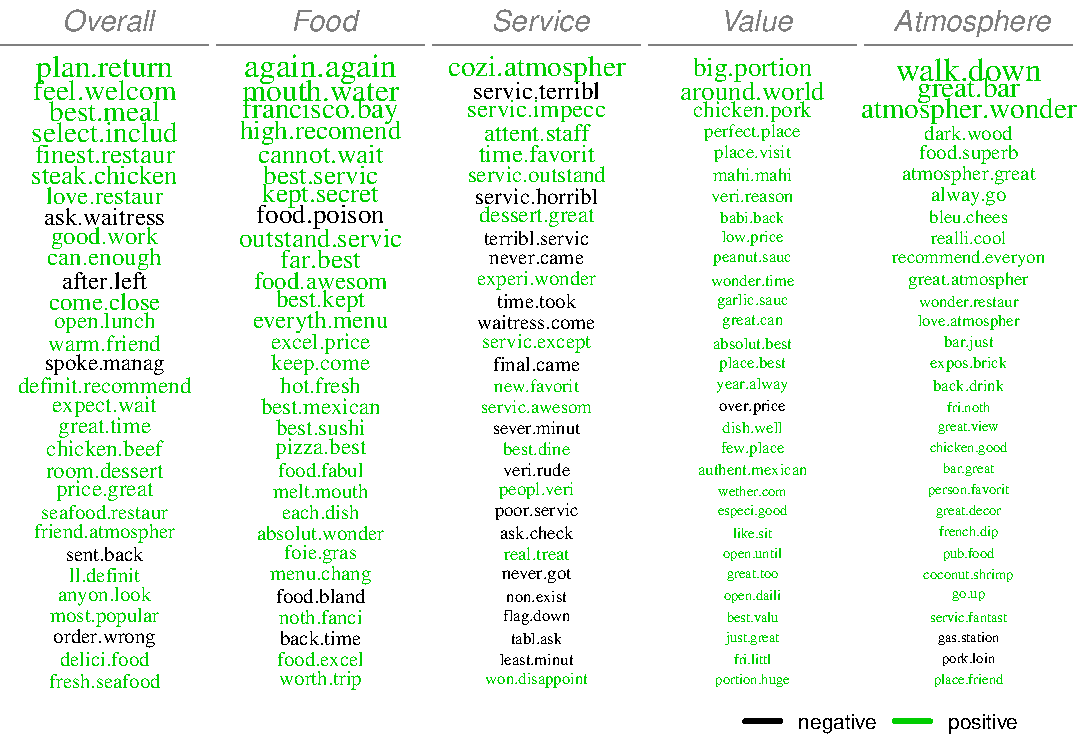
\includegraphics[width=4.35in]{we8thereLoads}
\vskip -.5cm
\end{frame}

\begin{frame}

{\bf Inverse Regression and Factor Models}


\sk
Recall our interpretation of Principal Components via Factors

\vskip .2cm
~~~~PCA(1) fits $\ds{E}[x_{ij}]= \varphi_{j1} v_{i1},~j=1...p$ \\
{\gr ~~~~~to minimize deviance over {\it both} rotations $\bs{\varphi}$ and factor $v_i$'s.}

\vskip .2cm
$1^{st}$ PC direction for observation $i$ is 
$\nv z_{i} = \bm{x}_i'\bs{\varphi} = \sum_{j=1}^p \varphi_{j} x_{ij}$

\sk
This is a projection from $\bm{x}$ into the space of the unknown $v$.

Beyond geometry, the easiest interpretation is to think of each
principal component $z_{i}$ as a re-scaled version of the factor
$v_{i}$.

\sk
{\theme Here, the factor $v_i$ that you `project on' is unknown.}
\end{frame}


\begin{frame}

{\bf Inverse Regression \gr (IR)}

\vskip .25cm
In IR, we know use $v_i = y_i$: the `factor' is our response!
\\ 
IR $\bs{\varphi}$ are thus analogous to PC rotations.


\vskip .25cm
Thus to do inverse regression for text,
\begin{itemize}
\item Estimate $\bs{\varphi}$ in MN logistic regression for $\bm{x}$ on $y$
\[ \vspace{-.25cm} \gr \bm{x}_i \sim \mr{MN}(\bm{p}_i, m_i)~~\text{with}~~\mr{p}_{ij} 
= \frac{\exp[\alpha_j +
y_i'\varphi_{j}]}{\sum_{l=1}^p \exp[\alpha_l 
+ y_i\varphi_{l} ]} \]
\item \vskip -.25cm Project $z_i = \bm{f}_i'\bs{\varphi}$ 
for all $i$ (i.e., $\bm{z} = \bm{F}\bs{\varphi}$)\\
{\gr Note that we use $\bm{f}$ for the projections here.}
\end{itemize}

\sk
Prediction is complete with a low-D `{\theme forward regression}'.\\
{e.g., $\ds{E}[y | z] = \alpha + \beta z$ via OLS, or logistic regression of $y$ on $z$.}

\end{frame}


\begin{frame}[fragile]

{\bf MNIR on the we8there reviews}

\vskip .25cm
{\footnotesize
\verb!summary( fitwe8 <- mnlm(we8thereCounts, y, bins=5) )!}


\vspace{-.5cm}
\begin{columns}


\column{1.5in}
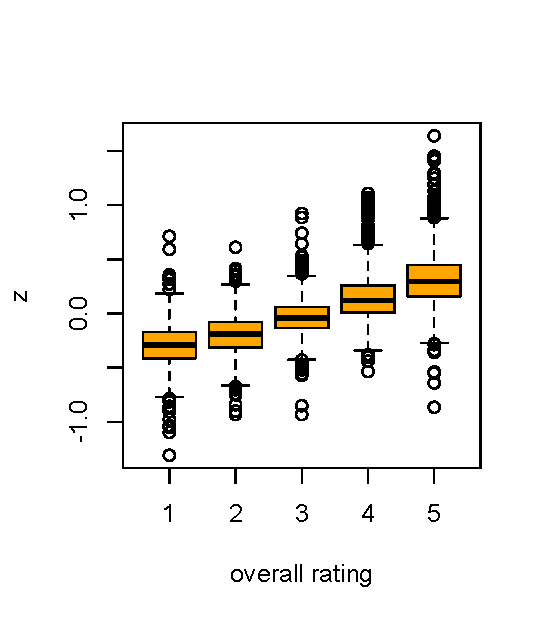
\includegraphics[width=1.75in]{../graphs/we8thereZ}

\column{2.5in}

{\tt \footnotesize

\theme \# first row is  intercepts\\
\nv phi = coef(fitwe8)[2,]

\theme \# sum(F[i,]*phi) for each row

\nv z <- F\%*\%phi 
}

\end{columns}

{\footnotesize \nv 
\begin{verbatim}
> summary(fwd <- glm(y~z))
            Estimate Std. Error t value Pr(>|t|)    
(Intercept)  3.50113    0.01343  260.63   <2e-16 ***
z            3.10047    0.03959   78.32   <2e-16 ***
\end{verbatim}}

{\small \gr So 0.3 increase in $z$ $\Rightarrow$ expected 1 star extra.}
\end{frame}



% \begin{frame}

% {\bf \theme
% Sentiment Analysis}


% \vskip .25cm
% A common task for text mining is to predict \\
% {\it sentiment} from speech/reviews/blogs/emails/etc.

% \vskip .25cm
% {\gr \it ~~~~~Sentiment about politicians in twitter traffic}
% 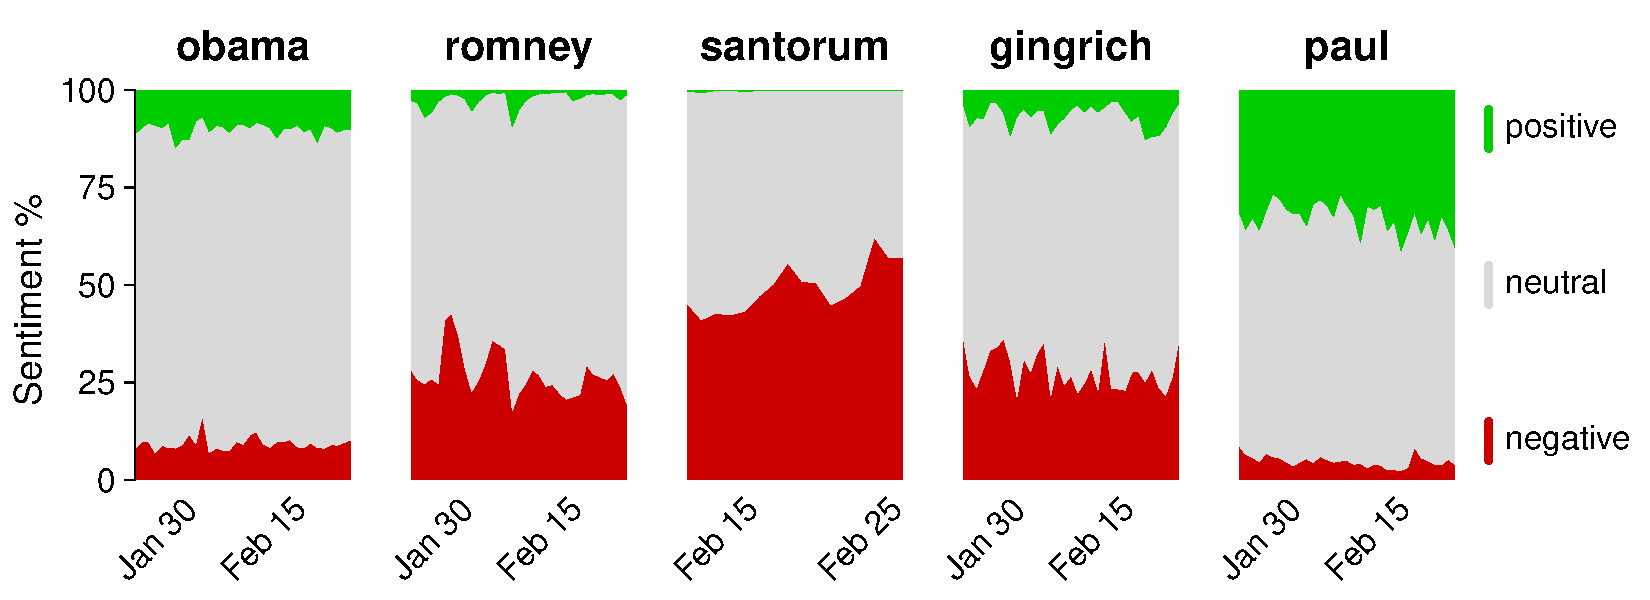
\includegraphics[width=4in]{../graphs/politicaltwitter}

% \vskip .25cm
% Sentiment is a very broad concept: \\
% happy/sad, positive/neutral/negative, willingness to pay, ...\\
% {\nv For data mining, it is only ever defined as what you measure.}


% \end{frame}

\begin{frame}

{\bf Roundup on \theme text mining}


\sk\bk
People work on language models beyond bag-of-words, \\but it
has previously  proven hard to make big improvements.\\
{\theme The state of the art is to tokenize and model counts.}

\sk
There are  fancy text specific models, but you can go a very long ways
using  generic data mining methods 
{\gr (esp. CV-lasso)}.  \\
MN (IR) models are just more efficient (do more with less).


\sk 
Text information is usually best as part of a larger system.

Use text data to fill in the cracks around what you know.

Don't ignore good variables with stronger signal than text!

\end{frame}

\end{document}
